\chapter{Power Analysis}
\graphicspath{{foto/Chap3/}}

The estimation of power consumption is based on the analytical power
model described in [1].

\section{Capacitance modeling}
The considered capacitances are the following:
\begin{itemize}
	\item $C_{g,fg}$ gate capacitance of floating gate transistor
	\item $C_{d,fg}$ "drain/source" capacitance of floating gate transistor
	\item $C_{g,pt}$ gate capacitance of a generic pass transistor (SST and GST)
	\item $C_{d,pt}$ "drain/source" capacitance of a generic pass transistor (SST and GST)
	\item $C_{g,rowpass}$, $C_{g,colpass}$ and $C_{g,slice}$gate capacitance of SET and column pass transistors
	\item $C_{d,rowpass}$, $C_{d,colpass}$ and $C_{d,slice}$ drain capacitance of SET, column and slice pass transistors 
	\item $C_{wl,wire}$ wire capacitance per unit length of wordline
	\item $C_{bl,wire}$ wire capacitance per unit length of bitline
	\item $C_{ssl,wire}$ wire capacitance per unit length of string select line (the same for ground select line)
	\item $C_{slice,dec},C_{row,dec},C_{col,dec}$ total capacitances of each type of decoder
	\item $C_{SA,in}$ $C_{SA}$ input and load capacitance of the sense amplifier
	\item $C_{g,pre}$ gate capacitance of the precharge transtistor
	\item $C_{ext,pu\_driver}$ external precharge unit driver capacitance
\end{itemize}

Other useful parameters are:

\begin{itemize}
	\item $N_{bl}$ number of bitlines 
	\item $N_{wl}$ number of wordlines
	\item $L_{bl}$ length of bitline 
	\item $L_{wl}$ length of wordline
	\item $N_{slice}$ number of slices
	\item $N_{erase}$ number of erase cycles
\end{itemize}

\subsection{Floating gate transistor capacitances}

To evaluate power dissipation of a Floating Gate Transistor, the values of its capacitances are needed.\\
While in a traditional MOS structure there are Source, Drain and Gate capacitances, in a FGT there is a double gate structure (floating gate and control gate): the two capacitances $C_{fg}$ and $C_{cg}$ can be modeled as a single equivalent gate capacitance $C_{g,fg}$, series of the two and then equal to:

\[
C_{g,fg}=\frac{C_{fg} \cdot C_{cg}}{C_{fg}+C_{cg}}
\]

\subsection{Lines capacitances}
\label{subsec:capacitance}

To accurately evaluate the capacitance of the lines ($C_{bl}$ and $C_{wl}$), the capacitance of the wires  and the length of bitline/wordline are considered. So the total capacitance for each line is:

\[
C_{wl} = C_{d,rowpass} + C_{g,fg} \cdot N_{bl} + C_{wl,wire} \cdot L_{wl}
\]

\[
C_{bl}=2 \cdot C_{d,pt}+N_{wl}\cdot C_{d,fg}+C_{bl,wire} \cdot L_{bl} +C_{SA,in}
\]

where $C_{SA,in}$ is the input capacitance of the sense amplifier
\subsection{Decoders capacitance}
\label{subsec:dec_capacitance}
To evaluate the capacitance of the decoders, the following formulas are used:
\[
C_{slice,dec}=C_{d,sdec,pcharge}+C_{d,sdec,eval}+C_{g,sdec,inv_{p}}+C_{g,sdec,inv_{n}}
\]

\[
C_{slice,stack}=0.5 \cdot C_{g,sdec,n} \cdot Block\_Address \cdot N_{slice};
\]

where $C_{g,dec,eval}, C_{d,sdec,pcharge}$ and $C_{d,sdec,eval}$ are, respectively, the gate/drain capacitance of the precharge and evaluation transistors, while the others are the gate capacitances of the output inverter.
In particular, $C_{d,sdec,eval} = Block\_Address \cdot C_{d,sdec,n}$.\\
$C_{slice,stack}$ is the equivalent gate capacitance, that has to be loaded to turn on the n-mos and select the correct output, given certain selection bits from the address.\\
Similar expressions have been used for row and column decoders.
\subsection{Sense Amplifier}
\label{subsec:dec_capacitance}
To evaluate the capacitance of the sense amplifier, the following formulas are used:
\[
C_{SA,in}=C_{d,sa,p}+C_{d,sa,n}+C_{g,sa,p}+C_{g,sa,n}
\]

\[
C_{SA}=C_{d,colpass}+C_{d,slice}
\]

\section{Read Dynamic Power}
\label{sec:read_power}
\subsection{Decoding stage}
\label{sec:decoding_stage}
During a read operation, the slice decoder selects the slice in which the operation has to be carried out.
At the same time other two decoders, the row and the column one, are working to select the addressed word.
The formulas to calculate energy consumption in the decoding phase are the following:
\[
E_{slice,dec}= 0.5 \cdot C_{slice,dec} \cdot V_{on,pt}^2
\]
\[
E_{stack,sdec}=0.5 \cdot C_{slice,stack} \cdot V_{on,pt}^2
\]

\[
E_{row,dec}= 0.5 \cdot C_{row,dec} \cdot (V_{rd,sel}^2+ V_{rd,unsel}^2 \cdot (N_{wl}-1) + 2 \cdot V_{on,pt}^2) \cdot N_{slice}
\]
\[
E_{stack,rdec}=0.5 \cdot C_{row,stack} \cdot V_{on,pt}^2 \cdot N_{slice}
\]

\[
E_{col,dec}= 0.5 \cdot C_{col,dec} \cdot V_{on,pt}^2 \cdot N_{slice}
\]
\[
E_{stack,cdec}=0.5 \cdot C_{col,stack} \cdot V_{on,pt}^2 \cdot N_{slice}
\]

In this analysis, we are making the assumption that all the decoders have the same structure, but in reality the page decoder has a more complex one, having to give different voltages in output for each wordline.\\
The energy consumption linked to the selection of the slice and of the columns can be expressed as:
\[
E_{row,pt}= 0.5 \cdot (C_{g,rowpass} \cdot (N_{wl}+2) + N_{bit,word} \cdot C_{g,slice} ) \cdot V_{on,pt}^2
\]

\[
E_{col,pt}= 0.5 \cdot N_{bit,word} \cdot C_{g,colpass} \cdot V_{on,pt}^2
\]

\subsection{Precharge}
\label{sec:precharge}
In this state all the lines are isolated from the memory array and the bitlines are biased to a specific value $V_{bl,prec}$, by the precharge block, to speed up the following operation in order to reduce the latency. The other lines are biased to ground.\\
The formulas to calculate dissipated energy in the precharge phase are the following:

\[
E_{pre}= 0.5 \cdot (C_{ext,pu\_driver}+C_{g,pre}) \cdot V_{bl,prec}^2 \cdot N_bl
\]

\[
E_{bl}= 0.5 \cdot C_{bl,wire} \cdot L_{bl} \cdot V_{bl,prec}^2 \cdot N_{bl}
\]

\subsection{Read operation}
\label{sec:read_op}

The wordline of the selected page is biased to ground ($V_{rd,sel}$) while the voltage on the insulated page is set to $V_{rd,unsel}$. In this way the unselected pages act as a transfer gates and are always on independently from the values stored in the FGTs. It is assumed that the initial voltage of the wordline is 0.\\

The energy to switch the selected wordline is the following:
\[
E_{sel}= 0.5 \cdot C_{wl} \cdot V_{rd,sel} ^2
\]

The energy to switch the unselected wordlines is:
\[
E_{unsel}= 0.5 \cdot C_{wl}  \cdot V_{rd,unsel}^2 \cdot (N_{wl}-1)
\]

The bitlines are at the precharge voltage $V_{bl,prec}$ and are connected to the strings using SSTs and GSTs. Depending on the threshold voltage of the FGTs (1 or 0 stored) in the selected page, the bitlines can have two different kinds of voltage drop, $V_{rd,1}$ and $V_{rd,0}$. So a parameter that considers the distribution of 0s and 1s stored in the memory is used ($p_0$).\\

The energy to read a 1 is:
\[
E_1=0.5 \cdot C_{bl} \cdot (V_{bl,prec}-V_{rd,1})^2 \cdot N_{bl} \cdot (1-p_0)
\]

The energy to read a 0 is:
\[
E_0=0.5 \cdot C_{bl} \cdot (V_{bl,prec}-V_{rd,0})^2 \cdot N_{bl} \cdot p_0
\]

where $V_{bl,prec}-V_{rd,0}$, $V_{bl,prec}-V_{rd,1}$ are the voltage swing to the read of '0' and '1'.\\
The energy to activate SST and GST is:
\[
E_{pt}= 2 \cdot [0.5 \cdot C_{G,pt} \cdot V_{on,pt}^2] \cdot N_{bl}
\]
where $V_{on,pt}$ is the voltage to enable the pass transistors.

The energy on the string select line and ground select  line is:
\[
E_{sl}=E_{ssl}+ E_{gsl} = 2 \cdot [0.5 \cdot (C_{ssl,wire}\cdot L_{wl}) \cdot V_{on,pt}^2]
\]

\subsection{Sense Amplifier}
\label{sec:sense_amp}

The state change in the bitline is detected using a sense amplifier connected to each line.
The energy consumption related to this stage is given by:

\[
E_{SA}= 0.5 \cdot C_{SA} \cdot V_{bl,prec} \cdot ((V_{bl,prec}-V_{rd,0}) \cdot p_0 + (V_{bl,prec}-V_{rd,1}) \cdot (1-p_0)) \cdot N_bl
\]


\subsection{Total Power}
\label{sec:total_power}

Total energy is computed as summation of all the previous terms.
Assuming $f_{read}$ as read frequency and $E_{read}$as total read energy,, total read power can be computed as follows:
\[
P_{read}=E_{read}\cdot f_{read}
\]

\section{Write Dynamic Power}
\label{sec:write_power}
In the write stage, only the cells where the logical 0s will be written must be programmed, the others need to be inhibited. This can be performed by applying a voltage on the bitline that is 80\% of the voltage on the control gate ($V_{inhibit}$). The bitlines that need to be programmed with logical 0 are biased to ground. On all the control gates of the page a program voltage ($V_{prog}$) is applied. There is also a contribute due to tunneling energy $E_{tunnel}$.  It is assumed that the precharge voltage of the wordline is 0.\\

For the writing operation the column decoding is unneeded, being the page the smallest programmable unit. 
So the energy consumption for the decoding stage is given, as before, by the relations: 

\[
E_{slice,dec}= 0.5 \cdot C_{slice,dec} \cdot V_{on,pt}^2
\]
\[
E_{stack,sdec}=0.5 \cdot C_{slice,stack} \cdot V_{on,pt}^2
\]

\[
E_{row,pt}= 0.5 \cdot(C_{g,rowpass} \cdot (N_{wl}+2) + N_{bit,word} \cdot C_{g,slice} ) \cdot V_{on,pt}^2
\]

\[
E_{row,dec}= 0.5 \cdot C_{row,dec} \cdot (V_{prog}^2 + V_{inhibit}^2 \cdot (N_{wl}-1) + 2 \cdot V_{on,pt}^2) \cdot N_{slice}
\]
\[
E_{stack,rdec}=0.5 \cdot C_{row,stack} \cdot V_{on,pt}^2 \cdot N_{slice}
\]

The energy to precharge the bitlines is:
\[
E_{pre}= 0.5 \cdot C_{g,pre} \cdot V_{bl,prec}^2 \cdot N_{bl}
\]

\[
E_{bl}= 0.5 \cdot C_{bl,wire} \cdot L_{bl} \cdot V_{bl,prec}^2 \cdot N_{bl}
\]

The energy to switch the selected wordline is:

\[
E_{sel}=0.5 \cdot C_{wl} \cdot V_{prog}^2
\]

The energy to switch the unselected wordlines is:

\[
E_{unsel}=0.5 \cdot C_{wl} \cdot V_{inhibit}^2 \cdot (N_{wl}-1)
\]

The inhibit energy to maintain 1 in the cells is:

\[
E_{bl,inhibit}=0.5 \cdot (C_{bl}-C_{d,fg} \cdot N_{wl})\cdot (0.8 \cdot V_{inhibit})^2 \cdot N_{bl} \cdot (1-p_0)
\]

According to the self-boosted program inhibit model, the channel voltage is boosted to about $80\%$ of the applied control gate voltage by biasing the bit-lines corresponding to logical 1 at a specific voltage, in order to have that the boosted channel voltage is a fraction of the applied control gate voltage ($0.8 \cdot V_{inhibit}$).\\

The energy to program (write a 0) is:

\[
E_{bl,sel}= ( 0.5 \cdot (C_{bl}-C_{d,fg} \cdot N_{wl}) \cdot (0-V_{bl,prec})^2 + E_{tunnel}) \cdot N_{bl} \cdot p_0 
\]
The program voltage to be applied to the bitline is 0.\\


The energy to activate the pass transistors is:
\[
E_{pt}= 2 \cdot [0.5 \cdot C_{G,pt} \cdot V_{on,pt}^2] \cdot N_{bl}
\]
The energy on the string select line and ground select  line is:
\[
E_{sl}=E_{ssl}+ E_{gsl} = 2 \cdot [0.5 \cdot (C_{ssl,wire}\cdot L_{wl}) \cdot V_{on,pt}^2]
\]


In conclusion, the total amount of energy for a write operation is given by the addition of all these terms.\\
Assuming $f_{write}$ as write frequency and $E_{write}$as total write energy, total write power can be computed as follows:

\[
P_{write}=E_{write}\cdot f_{write}
\]


\section{Erase power}
\label{sec:erase_power}
For the erase operation, in planar flash NAND, the well of the block to erase is biased to an high voltage and the control gates are connected to ground. A high voltage is applied on the bitlines ($V_{prog}$) and the gates are biased to ground to have a tunnel effect that is in the opposite direction with respect to the write case. Also in this instance the tunnel energy must be considered.\\

Even in this case, the column decoding is unneeded and so the energy consumption is given, as before, by the relations: 

\[
E_{slice,dec}= 0.5 \cdot C_{slice,dec} \cdot V_{on,pt}^2
\]
\[
E_{stack,sdec}=0.5 \cdot C_{slice,stack} \cdot V_{on,pt}^2
\]

\[
E_{row,pt}= 0.5 \cdot (C_{g,rowpass} \cdot (N_{wl}+2) + N_{bit,word} \cdot C_{g,slice} ) \cdot V_{on,pt}^2
\]

\[
E_{row,dec}= 0.5 \cdot C_{row,dec} \cdot (V_{bl,erase}^2 \cdot N_{wl} + 2 \cdot V_{on,pt}^2) \cdot N_{slice}
\]
\[
E_{stack,rdec}=0.5 \cdot C_{row,stack} \cdot V_{on,pt}^2 \cdot N_{slice}
\]
The precharge step is required:
\[
E_{pre}= 0.5 \cdot C_{g,pre} \cdot V_{bl,prec}^2 \cdot N_bl
\]

\[
E_{bl}= 0.5 \cdot C_{bl,wire} \cdot L_{bl} \cdot V_{bl,prec}^2 \cdot N_{bl}
\]
The energy necessary to start erasing the block is:


\[
E_{erase,slice}=0.5 \cdot C_{bl} \cdot (V_{bl,erase}-V_{bl,prec})^2 \cdot N_{bl}+E_{tunnel} \cdot N_{bl} \cdot N_{wl}
\]
where $E_{tunnel} \cdot N_{bl} \cdot N_{wl}$ is the tunneling energy for the block.\\
The energy to activate the two pass transistors is the following:
\[
E_{pt}= 2 \cdot [0.5 \cdot C_{G,pt} \cdot V_{on,pt}^2] \cdot N_{bl}
\]

The energy on the string select line and ground select  line is:
\[
E_{sl}=E_{ssl}+ E_{gsl} = 2 \cdot [0.5 \cdot (C_{ssl,wire}\cdot L_{wl}) \cdot V_{on,pt}^2]
\]


Total energy for the erase operation is:

\[
E_{erase}=E_{slice,dec}+E_{stack,sdec}+E_{row,pt}+E_{stack,rdec}+E_{row,dec}+E_{bl}+(E_{erase,slice}+E_{pt}+E_{sl}) \cdot N_{erase}
\]	
where $N_{erase}$ is the number of erase cycles, necessary for the operation to be performed correctly.\\
Assuming $f_{erase}$ as erase frequency, total erase power can be computed as follows:
\[
P_{erase}=E_{erase}\cdot f_{erase}
\]

\section{Simulation results}
To verify the plausibility of our computations we assigned a reasonable value to each of the parameters involved in the equations.\\
In a first simulation the number of wordlines and bitlines change in a well defined range, to analyse how the power consumption changes if we vary the dimensions of the memory array. In particular, the array of values we considered for both $N_{wl}$ and $N_{bl}$, as for the delay, is $[64, 128, 256, 512, 1024, 2048]$. For each simulation point we assumed that $N_{bl}=N_{wl}$, because usually the memory arrays are made as square as possible, for reasons of space availability on the board.\\

The obtained results are reported in the following figures. 

\begin{figure}[H] 
	\begin{center}
		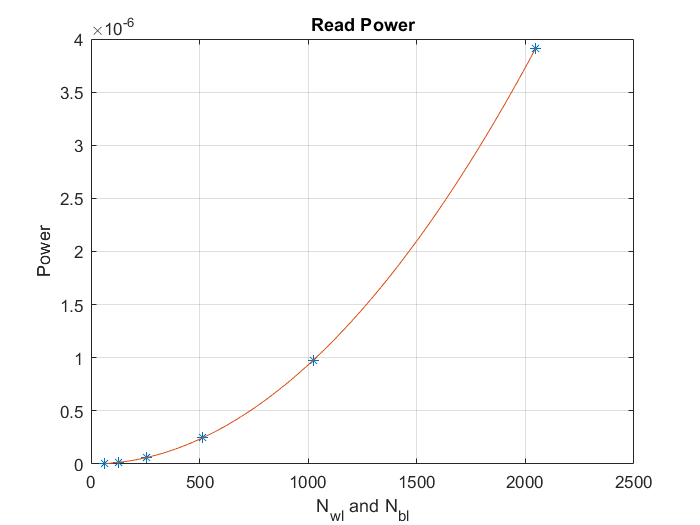
\includegraphics[scale=0.4]{Read_power_bl}
		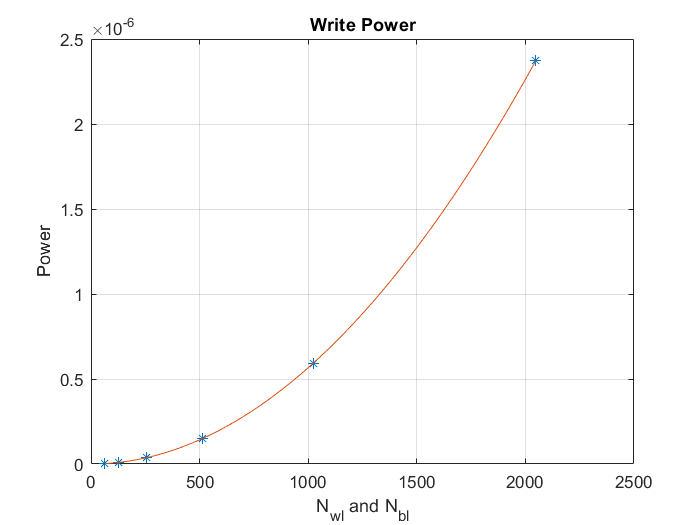
\includegraphics[scale=0.4]{Write_power_bl}
	\end{center}
	\caption{Read Dynamic Power and Write Dynamic Power versus $N_{wl},N_{bl}$}
	\label{readwrite}
\end{figure}

\begin{figure}[H] 
	\begin{center}
		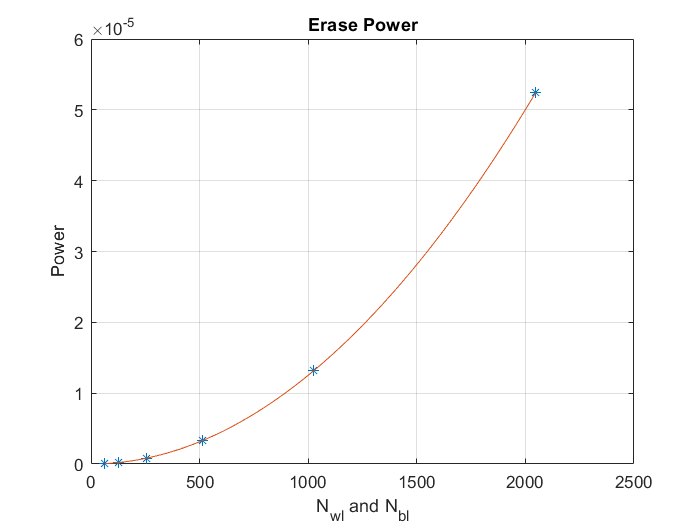
\includegraphics[scale=0.4]{Erase_power_bl}
	\end{center}
	\caption{Erase Dynamic Power versus $N_{wl},N_{bl}$}
\end{figure}

The behaviour represented is reasonable: in all the contributions previously discussed there is a more than linear dependence on $N_{wl}$ and $N_{bl}$. In particular the most relevant contributions are dependent from the product of these two parameters, giving as result a quadratic curve.\\
The curves in Figure \ref{readwrite} show that power consumption for read and write operations is in the order of some $\mu W$, while the erase power is about one order of magnitude larger.\\
In a second analysis $N_{wl}$ and $N_{bl}$ are fixed, with a value of 1024, while $N_{slice}$ varies according to the values $[32, 64, 128, 256]$.
\begin{figure}[H] 
	\begin{center}
		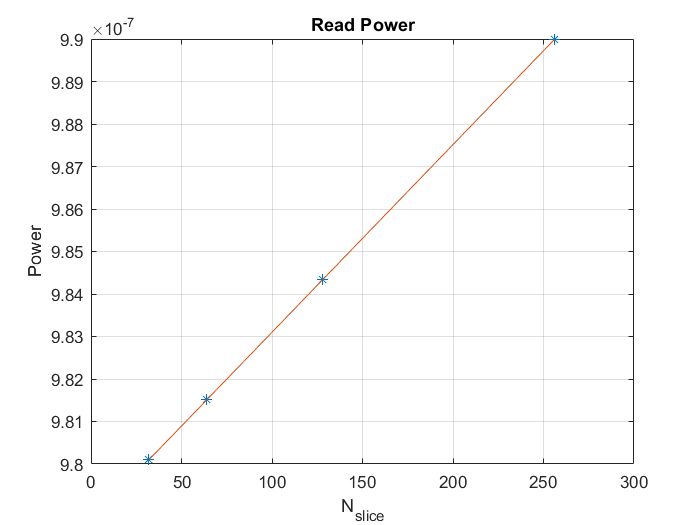
\includegraphics[scale=0.4]{Read_power_slice}
		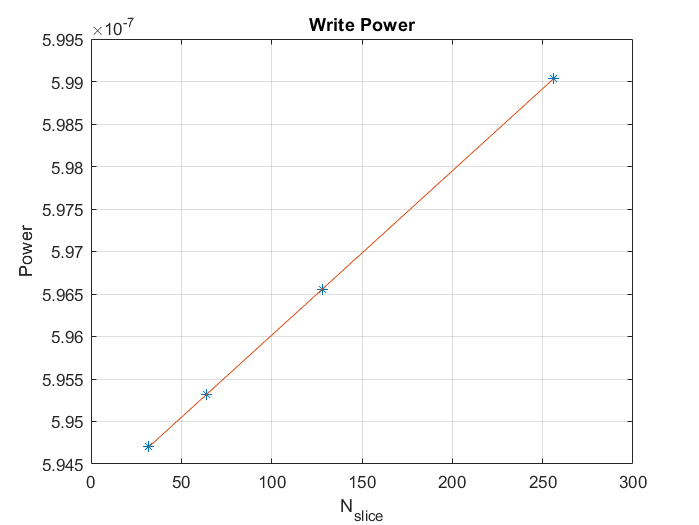
\includegraphics[scale=0.4]{Write_power_slice}
	\end{center}
	\caption{Read Dynamic Power and Write Dynamic Power versus $N_{slice}$}
\end{figure}

\begin{figure}[H] 
	\begin{center}
		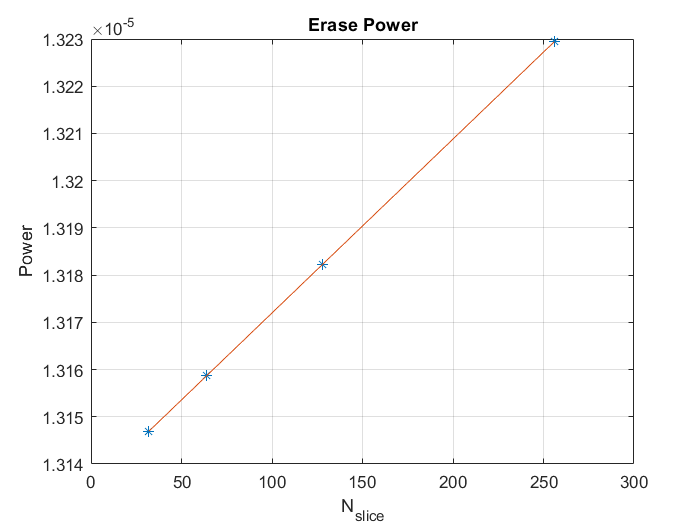
\includegraphics[scale=0.4]{Erase_power_slice}
	\end{center}
	\caption{Erase Dynamic Power versus $N_{slice}$}
\end{figure}

As it can be seen, the dependency from $N_{slice}$ is linear. However, having supposed that all the unselected blocks are deactivated, the increase in the curves is due to the power consumption of an higher number of decoders.